% Preamble
\documentclass[a4paper, 12pt]{article}
\usepackage{titlesec}
\usepackage[margin=0.5in]{geometry}
\usepackage{pdfpages}
\usepackage{amssymb}
\newcommand{\qed}{\\\ensuremath{\\\blacksquare}}
\titlelabel{\thetitle.\quad}

% Document
\begin{document}


% Title Page
\begin{titlepage}
    %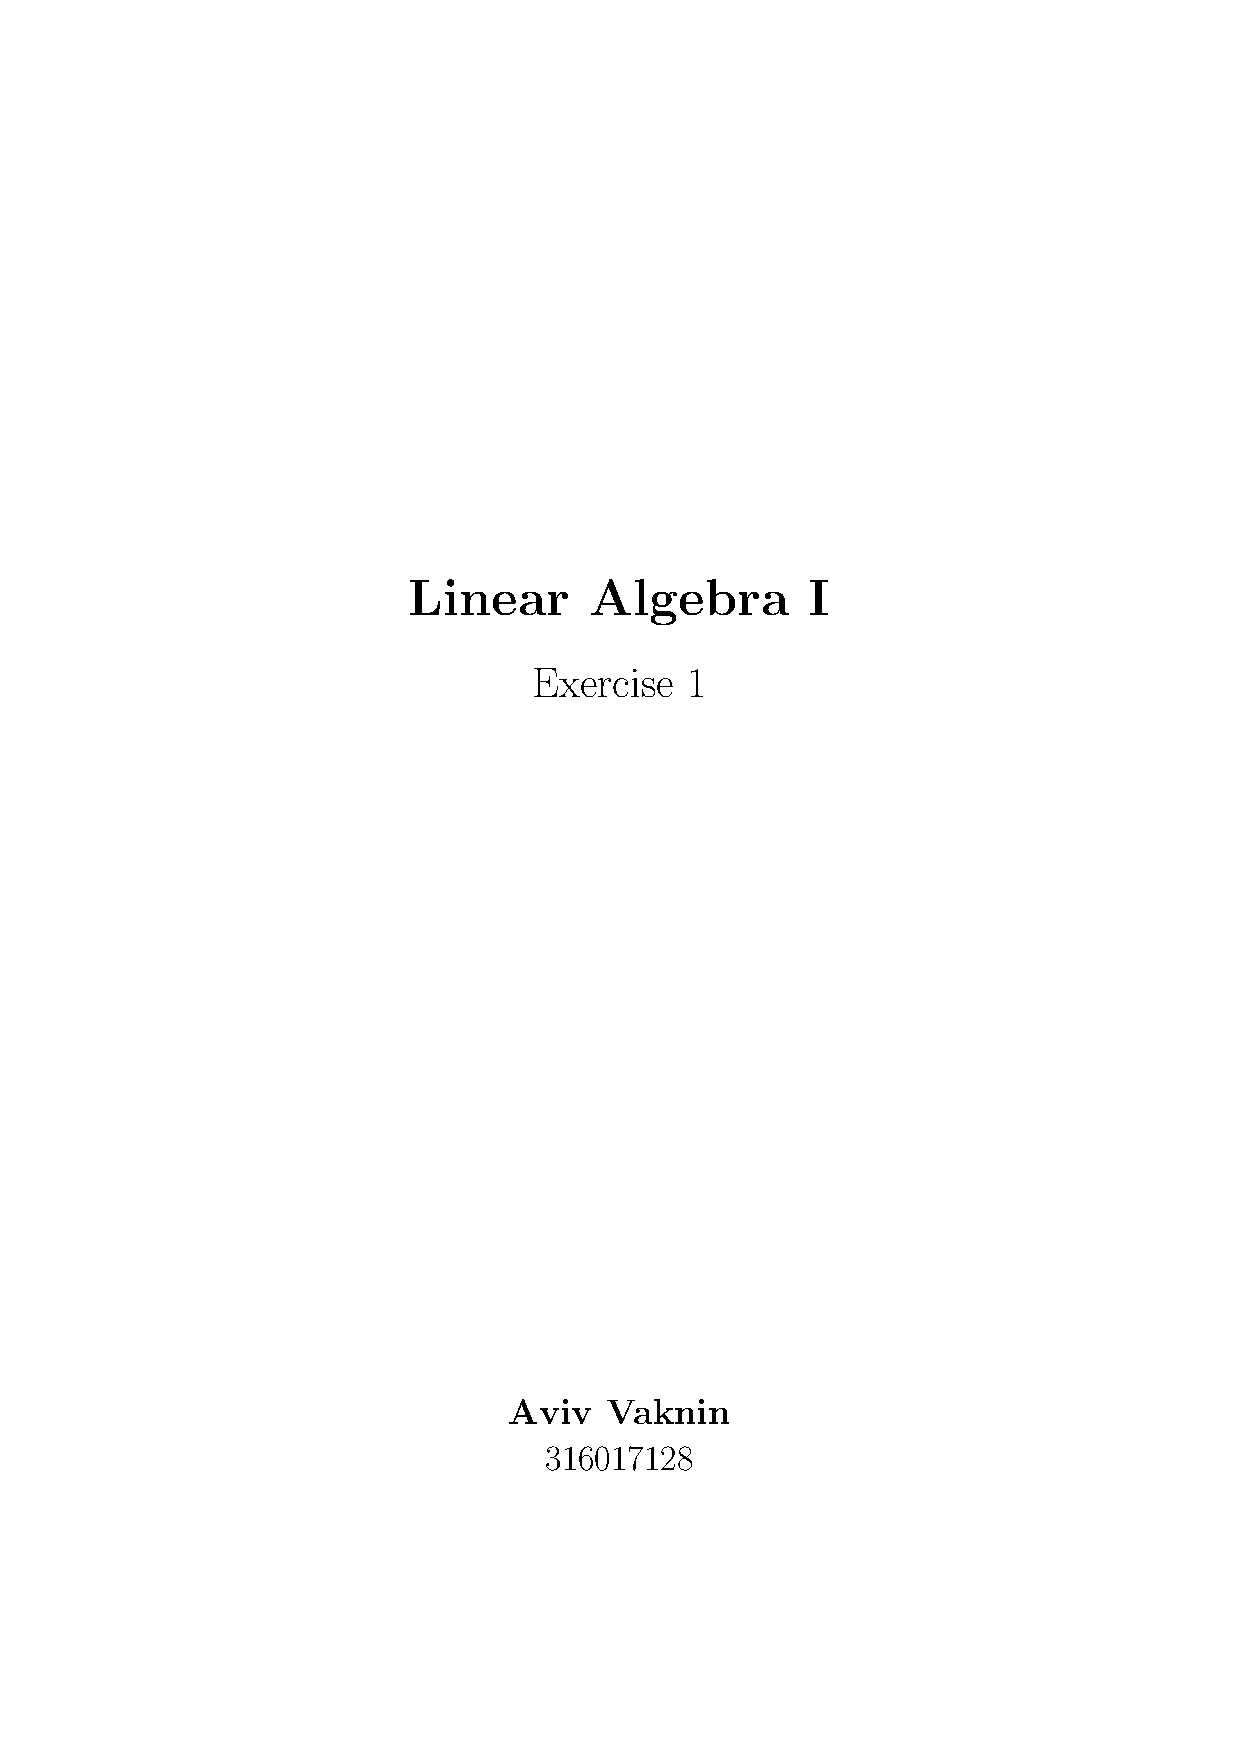
\includepdf{title.pdf}
\end{titlepage}

% 1
\section{}
In order to show that $S$ is a field, we'll need to prove the following \textit{\textbf{binary operator}} properties:
\begin{enumerate}
    \item In $S$, there are two members, zero - $0_S$ and one - $1_S$
    \item $S$ supports the addition and multiplication binary operators
    \item Every member in $S$ can be negated, i.e. for every $x$ there is $-x$
    \item For every member in $S$ that is not $0_S$, $\exists{x^{-1}}\in{S}$, it is called the multiplicative inverse of $x$
\end{enumerate}
In addition, the mentioned binary operators should satisfy the following properties, referred to as \textit{\textbf{field axioms}}:
\begin{enumerate}
    \item Associativity of addition(A1) and multiplication(M1):
        $$ a+(b+c)=(a+b)+c $$
        $$ a\cdot(b\cdot{c})=(a\cdot{b})\cdot{c} $$
    \item Commutativity of addition(A2) and multiplication(M2):
        $$ a+b = b+a $$
        $$ a\cdot{b} = b\cdot{a} $$
    \item Additive identity(A3) and multiplicative identity(M3)
        $$ a+0=a $$
        $$ a\cdot{1}=a $$
    \item Additive inverse(A4) and multiplicative inverse(M4)
        $$ a + (-a) = 0 $$
        $$ a \cdot a^-1 = 1 $$
    \item Distributivity(D)
        $$ a(b + c) = (a \cdot{b})+(a \cdot{c}) $$
\end{enumerate}
\pagebreak

% 2
\section{}
Prove: $ ((a + b) + c) + d = (a + b) + (c + d) = a + (b + (c + d)) $
\qed


\end{document}